\documentclass{sig-alternate}

\usepackage{url}
\usepackage{subfig}
\usepackage{tabularx}
\newcolumntype{R}{>{\raggedleft\arraybackslash}X}
\usepackage{siunitx} % provides \SI{}{\celsius} etc.
\usepackage{etoolbox}
\robustify\bfseries \sisetup{detect-weight = true}
\usepackage[numbers,square]{natbib}
\usepackage[affil-it]{authblk}
\usepackage{capt-of}
\usepackage{amsfonts}
\usepackage{tabularx}
\usepackage{cleveref}
\usepackage{booktabs}
\usepackage{microtype}
\usepackage{bbding}
\usepackage[noend]{algpseudocode}
\usepackage{algorithm}
%\usepackage{algorithmic}

\usepackage{balance}


\algnewcommand\algorithmicforeach{\textbf{for each}}
\algdef{S}[FOR]{ForEach}[1]{\algorithmicforeach\ #1\ \algorithmicdo} 
\def\BState{\State\hskip-\ALG@thistlm} 
 
\newcommand{\TRUE}{\textbf{true~}}
\newcommand{\FALSE}{\textbf{false~}}
\newcommand{\Break}{\textbf{break~}}
\newcommand{\Downto}{\textbf{down~to~}}


\newcommand\numberthis{\addtocounter{equation}{1}\tag{\theequation}}
\newcommand*\mean[1]{\bar{#1}}
\usepackage{color}
\usepackage[dvipsnames]{xcolor}

\newcommand{\commentBodo}[1]{{\color{blue}[BB thinks: {\emph{#1}}]}}
\newcommand{\etal}{et~al.}

% for table alignment
\newcommand{\Z}{\hphantom{0}}
\newcommand{\ZZ}{\hphantom{00}}
\newcommand{\ZZZ}{\hphantom{000}}
\newcommand{\ZZZZ}{\hphantom{0000}}
\newcommand{\ZZZZZ}{\hphantom{00000}}
\newcommand{\ZZZZZZ}{\hphantom{000000}}
\raggedbottom


\usepackage{color}
\newcommand{\todo}[1]{{\color{blue}[[TODO: {\emph{#1}}]]}}
\newcommand{\hopefully}{{\color{green}Hopefully: }}
\newcommand{\dave}[1]{{\color{green}[[Dave: {\emph{#1}}]]}}
\newcommand{\todoVthree}[1]{{\color{red}[[Bodo: {\emph{#1}}]]}}
\newcommand{\todoVfour}[1]{{\color{red}[[Thoughts: {\emph{#1}}]]}}
\newcommand{\todoVfive}[1]{{\color{magenta}[[Musings: {\emph{#1}}]]}}
\newcommand{\todoVsix}[1]{{\color{cyan}[[Ruminations: {\emph{#1}}]]}}
\newcommand{\LB}{\textsc{List building~}}
\newcommand{\LT}{\textsc{List traversal~}}
\newcommand{\script}[1]{$\mathcal{#1}$}


\newcommand{\AS}{Small Popular Query Set}
\newcommand{\TRECAP}{TREC-AP}
\newcommand{\TopQ}{Popular queries}
\newcommand{\classificationPaper}{Song lyrics}
\newcommand{\Wikipedia}{Wikipedia titles}
\newcommand{\AcademicID}{Academic paper titles}
\newcommand{\clueWebTitles}{ClueWeb12 titles}
\newcommand{\clueWebBodiesLarge}{ClueWeb12 bodies}
\newcommand{\Tweets}{Tweets}
\newcommand{\IndriWT}{Indri-WT10g}

\newcommand{\numcolls}{ten}

\newcommand{\PPold}{../../../BIGIR/RelevanceSciences/bodob/papers/syntheticCollection/Imagefiles}
%\newcommand{\PP}{../Experiments_emulation}
\newcommand{\PPS}{../From_Relsci/Experiments_sampling}
%\newcommand{\PPS}{../Experiments_sampling}

\title{Modelling term dependence}
\author{David Hawking
Bodo Billerbeck
Nick Craswell
Paul Thomas\\
Microsoft}

\begin{document}
\maketitle{}

\begin{abstract}

\end{abstract}

\section{Introduction}   %%%%%%%%%%%%%%% S1 %%%%%%%%%%%%%%%%



\section{Models of corpus growth}  %%%%%%%%%%%%%% S7 %%%%%%%%%%%%%%
\label{GrowthModels}

\begin{table}
\centering
\label{samples}
\begin{tabular}{l|lllllll}
\hline
Sample size & 1\% & 2\% & 5\% & 10\% & 20\% & 50\% & 100\%\\
No. samples & 7 & 6 & 5 & 4 & 3 & 2 & 1\\
\hline
\end{tabular}
\caption{Details of sample sizes used in studying collection growth.
\label{t:samples}}
\end{table}

We would like to provide a valid basis on which studies of algorithm
scalability could include synthetic corpora many times larger
than a base corpus.  In other words, to extract the model parameter values from a
base corpus and use a growth model to predict what the values of those
parameters would be if the corpus were scaled up by a factor of $k$.

In the absence of a better alternative, we assume that the base corpus
is an unbiased sample of an infinite parent corpus.  Scaling up the
base corpus by a factor of $k$ can be seen as drawing a sample $k$
times as large from the parent.

With this in mind, we derived growth models by randomly sampling
records from each base corpus to create samples ranging from 1\% to
100\% of the original.  We drew multiple samples of each size and took
the average of the parameter values for each size. The smaller the
sample size, the more samples we averaged.  We then plotted the change
in value of each parameter for each base corpus against sample size and 
determined, by inspection, the nature of the relationship.  These
relationships are tabulated in Table \ref{dynmodparams}.
Unsurprisingly, the mean and standard deviation of document length
don't change with change in sample size.  More interestingly, the
proportion of term occurrences accounted for by the ten highest
frequency terms also remains more or less constant.  Obviously,
the number of postings grows linearly with sample size.  Three
parameters related to the vocabulary size grow in proportion to a
fractional power of the scale up factor.  Power law growth in
vocabulary size is consistent with laws due to Herdan and Heaps. 


\begin{table}
\begin{tabular}{lll}
Parameter & Growth function & Additional information\\
\hline
$H_1\ldots H_{h}$&constant&\\
$s$&$s \times G^{\beta_1}$&$\beta_1$: mean = 0.155\\
&& st.~dev.~= 0.0938.\\
$\alpha$&$\alpha \times G^{\beta_2}$&$\beta_2$: mean = 0.0266\\
&& st.~dev.~= 0.0134.\\
$P$&linear & \\
$|V|$& $|V| \times G^{\beta_3}$&$\beta_3$: mean = 0.620\\
&& st.~dev.~= 0.125.\\
$\mathit{dl}$ mean & constant & \\
$\mathit{dl}$ st.~dev. & constant & \\
\hline
\end{tabular}
\caption{Corpus growth model. The parameters are the same as
  for the static model with $s=1, h=10$ but here we show how they vary as the corpus sample
  size increases.  $G$ is the factor by which the sample size is increased.
\label{dynmodparams}}
\end{table}


When simulating the growth of a base corpus, it would be most
convenient to avoid the need to derive a corpus-specific growth model
from samples.  Accordingly, we carried out scale-up experiments using
both corpus-specific models and a generic model averaged over the
\numcolls~ corpora.  Our growth model was developed using $h=10, s=1$.
Time has not permitted growth modeling of $S$, the 4-tuples describing
each piecewise segment.  This remains for future work.

\begin{figure*}[!ht]
\centering
   \subfloat[][Highest bigram frequency]{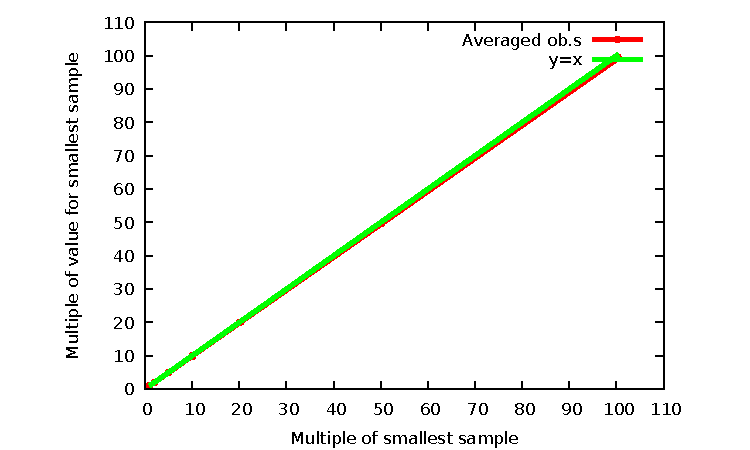
\includegraphics[width=0.505\textwidth]{\PPS/SamplePlots/scaling_TREC-AP_highest_bigram_freq.pdf}}
   \subfloat[][Total distinct
     bigrams]{\includegraphics[width=0.505\textwidth]{\PPS/SamplePlots/scaling_TREC-AP_total_bigrams.pdf}}
   
   \subfloat[][Significant distinct
     bigrams]{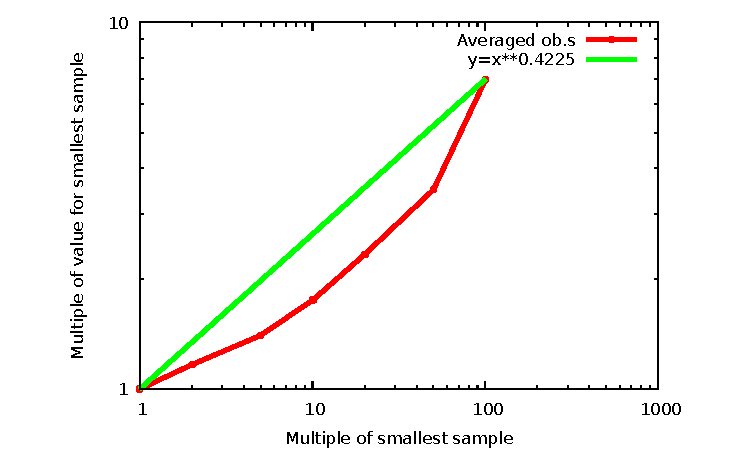
\includegraphics[width=0.505\textwidth]{\PPS/SamplePlots/scaling_TREC-AP_significant_bigrams.pdf}}
   \subfloat[][Bigram alpha]{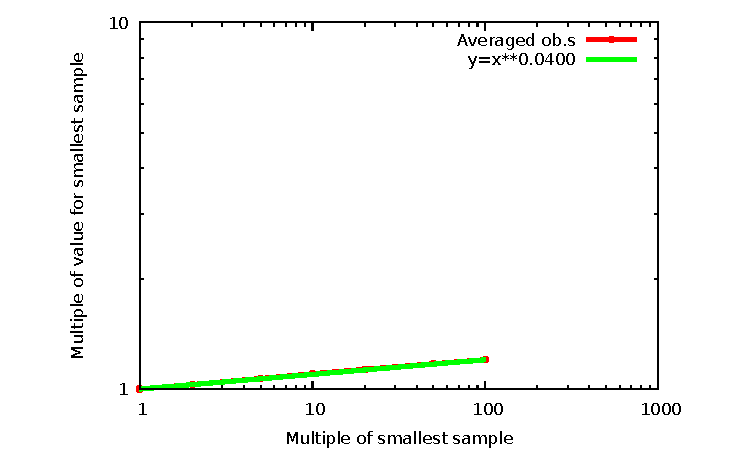
\includegraphics[width=0.505\textwidth]{\PPS/SamplePlots/scaling_TREC-AP_bigram_alpha.pdf}}
   
\caption{Showing how bigram attributes of a corpus change with
  growth in corpus size for the \TRECAP~corpus.  Note that subfigure
  (a) is a linear plot while the others are log log.
  \label{scalingup_bigrams_TA}}
\end{figure*}


\begin{figure*}[!ht]
\centering
   \subfloat[][Highest bigram frequency]{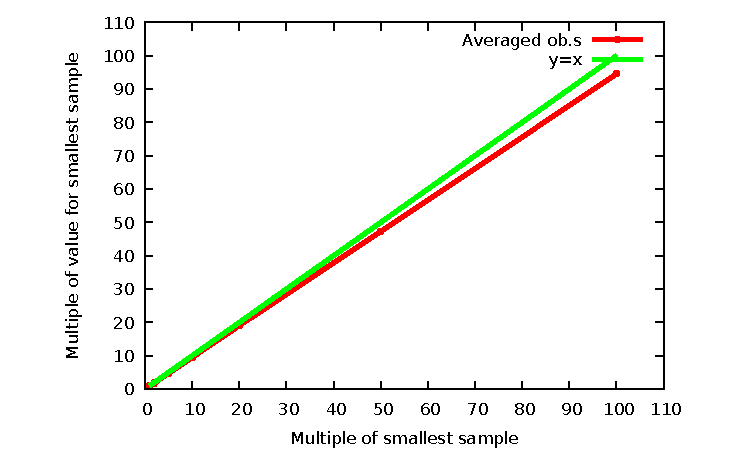
\includegraphics[width=0.505\textwidth]{\PPS/SamplePlots/scaling_Indri-WT10g_highest_bigram_freq.pdf}}
   \subfloat[][Total distinct
     bigrams]{\includegraphics[width=0.505\textwidth]{\PPS/SamplePlots/scaling_Indri-WT10g_total_bigrams.pdf}}
   
   \subfloat[][Significant distinct
     bigrams]{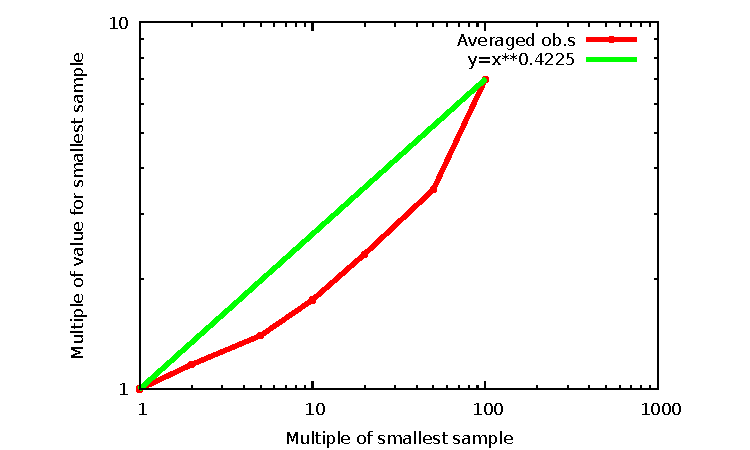
\includegraphics[width=0.505\textwidth]{\PPS/SamplePlots/scaling_Indri-WT10g_significant_bigrams.pdf}}
   \subfloat[][Bigram alpha]{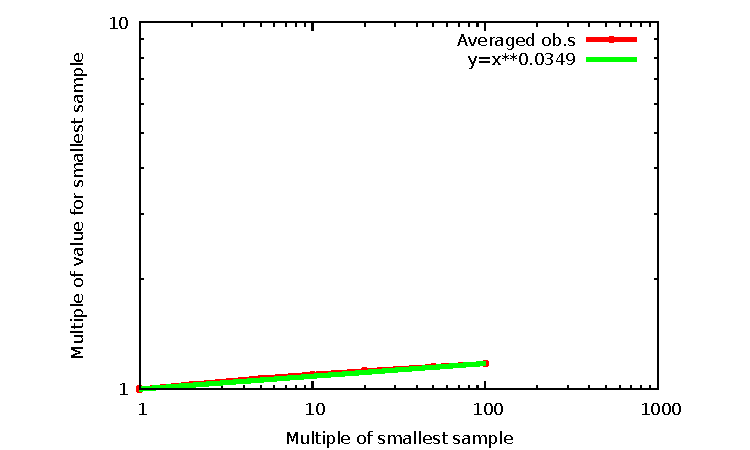
\includegraphics[width=0.505\textwidth]{\PPS/SamplePlots/scaling_Indri-WT10g_bigram_alpha.pdf}}
   
\caption{Showing how bigram attributes of a corpus change with
  growth in corpus size for the \IndriWT~corpus.  Note that subfigure
  (a) is a linear plot while the others are log log.
  \label{scalingup_bigrams_WT}}
\end{figure*}



\subsection{Effects of corpus growth on term dependency}

The discussion in the previous section and Figure~\ref{1-100} relate
to growth modeling with an assumption of word independence.  In this
section we start to look at how word dependence changes with increase
in corpus size.

Since we have modeled only n-gram associations in corpus emulations,
we start with that here.  The left hand plot in Figure~\ref{scalingup_bigrams_TA} suggests that 
the frequency of bigrams existing in a sample corpus grows linearly
with sample size. \todo{Can we confirm this in the shape of the
  distributions for different sample sizes?} The plots for the other
bigram parameters suggest a power law relationship.  These
observations are confirmed in the group of plots for \IndriWT.

The definition of ``significant bigram'' has been explained in the
section on emulation.



\section{Scaling up experiments}  %%%%%%%%%%%%%%% S9 %%%%%%%%%%%%%%%
\label{SUExpts}

\begin{figure*}[!ht]
\centering
   \subfloat[][Corpus specific: \TRECAP]{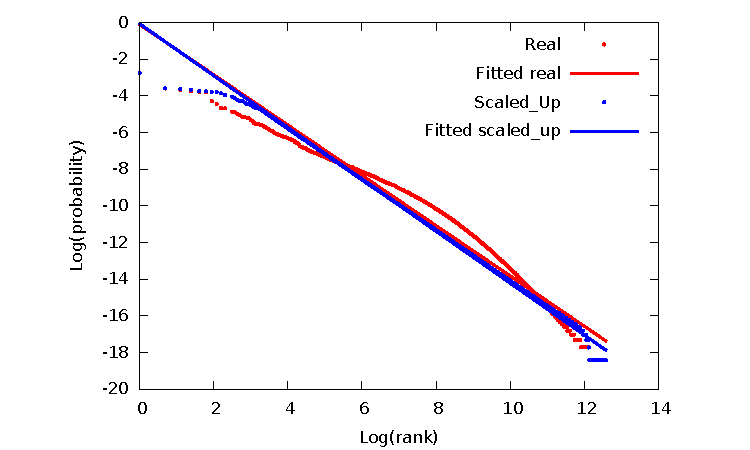
\includegraphics[width=0.505\textwidth]{\PPold/ScaledUpPlots/TREC-AP_real_v_scaled_up.pdf}}
   \subfloat[][Corpus specific: \Tweets]{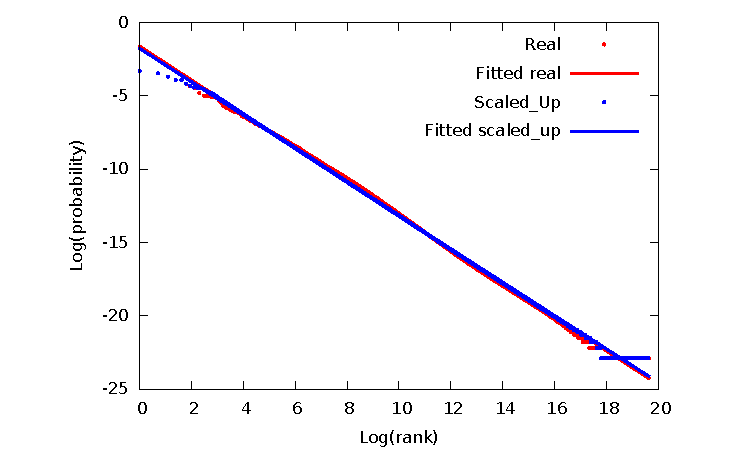
\includegraphics[width=0.505\textwidth]{\PPold/ScaledUpPlots/Tweets_real_v_scaled_up.pdf}}

   \subfloat[][Generic: \TRECAP]{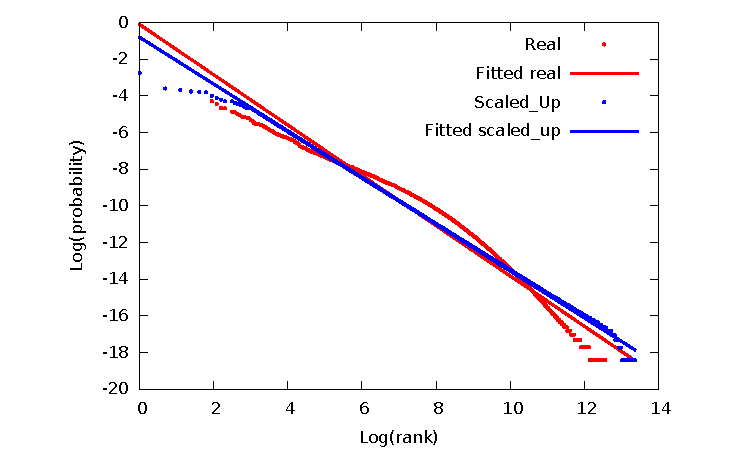
\includegraphics[width=0.505\textwidth]{\PPold/ScaledUpPlots/TREC-AP_real_v_generic_scaled_up.pdf}}
   \subfloat[][Generic: \Tweets]{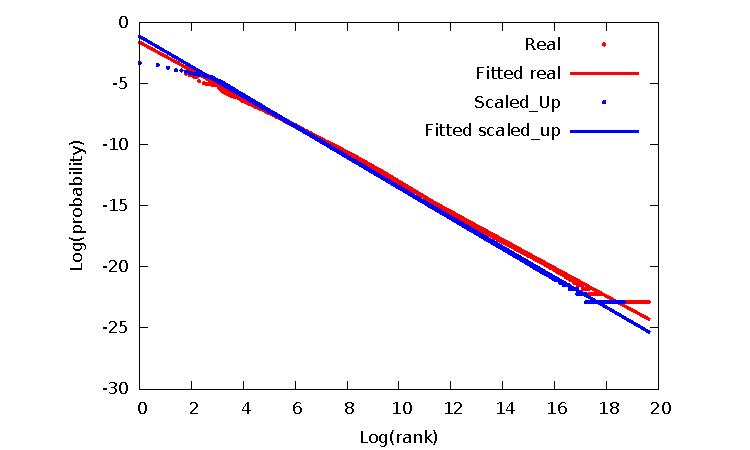
\includegraphics[width=0.505\textwidth]{\PPold/ScaledUpPlots/Tweets_real_v_generic_scaled_up.pdf}}
\caption{Emulating a corpus from a 1\% sample using growth models.
  The top row shows term probability distributions for corpus-specific 
  growth models and the bottom row shows those for a generic model. 
  Corpus \Tweets~was selected to illustrate a very close to linear 
  model while \TRECAP~is a corpus with very noticeable non-linearity.  \label{1-100}}
\end{figure*}



The scaling-up results are presented in Figure~\ref{1-100}.
They show that when \script{E} is derived from \script{C} using the
generic model the emulation is reasonable, though limited by the
accuracy of the linear static model.  Results for the \Tweets~ corpus,
whose term probability distribution is close to linear, are much
better than for \TRECAP.  If it proves feasible to derive
a good growth model for the piecewise case, we expect the results
to be much better for the corpora whose term probability distribution 
deviates substantially from linear. 

Note that the results in Figure~\ref{1-100} represent extrapolation
by two orders of magnitude, and that the base for extrapolation in 
some cases is quite small.  We expect that fidelity would be better
if the scale-ups were based on larger samples, say 10\%.






%%\nocite{*}

\bibliographystyle{abbrvnat}
\bibliography{p}
\end{document}
